The product is a multi functional application, where the main focus is to get knowledge about fishing and acquiring access to fishing areas in foreign places. 
The users of this application is divided into two groups: customers and shops. 

\subsection{The Customers}
The application provides knowledge for the customers by providing a platform, where it is possible to see a map with fishings areas, near the customer.

It provides a way to rent equipment, in case the customer does not have any or didn’t bring their equipment. 

The platform makes it easy to update or buy a fishing card and harder to forget, by saving it in the application. If the customer is a first time fisher or simply out of shape, there is a guide in the application, with tips and tricks, e.g.; How to tie a knot for the hook or information about which kind of fish is in season for catching. 

In case the customer has equipment, which he/she no longer uses, the platform provides a place for renting out the equipment.

The platform also provides a social aspect, where fishers can upload their catches. 


\subsection{The Shops}
The shops gets an opportunity to post their offers on the app and rent out their equipment.

\subsection{Software Requirements Specification for Application}

\begin{figure*}[t!]
  \centering
  \hfill
  \begin{subfigure}[t]{0.2\textwidth}
  	  \centering
  	  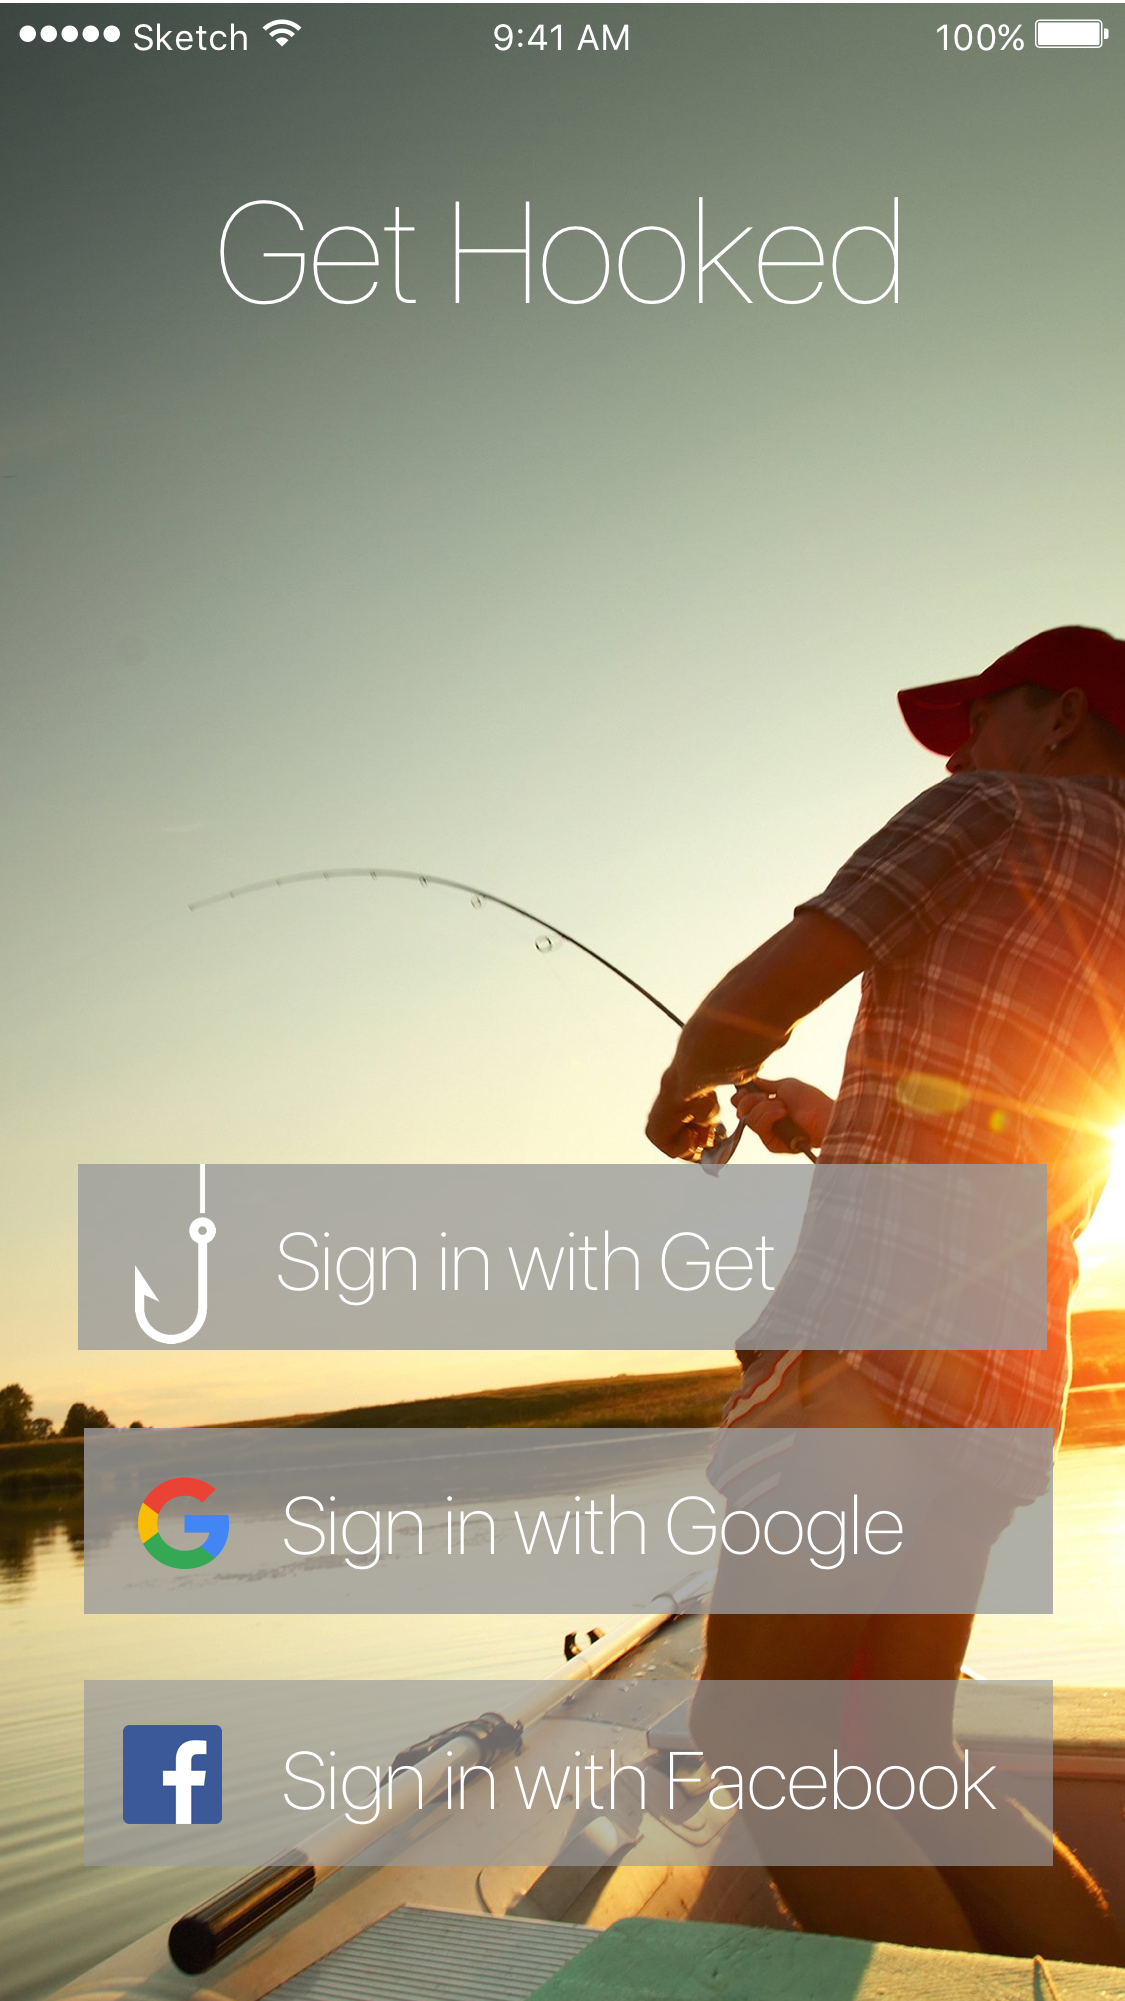
\includegraphics[width=0.4\textwidth]{images/Introscreen.png}
  	  \label{fig:f1}
  	  \caption{Single sign on screen}
  \end{subfigure}
  \hfill
  \begin{subfigure}[t]{0.2\textwidth}
  	  \centering
  	  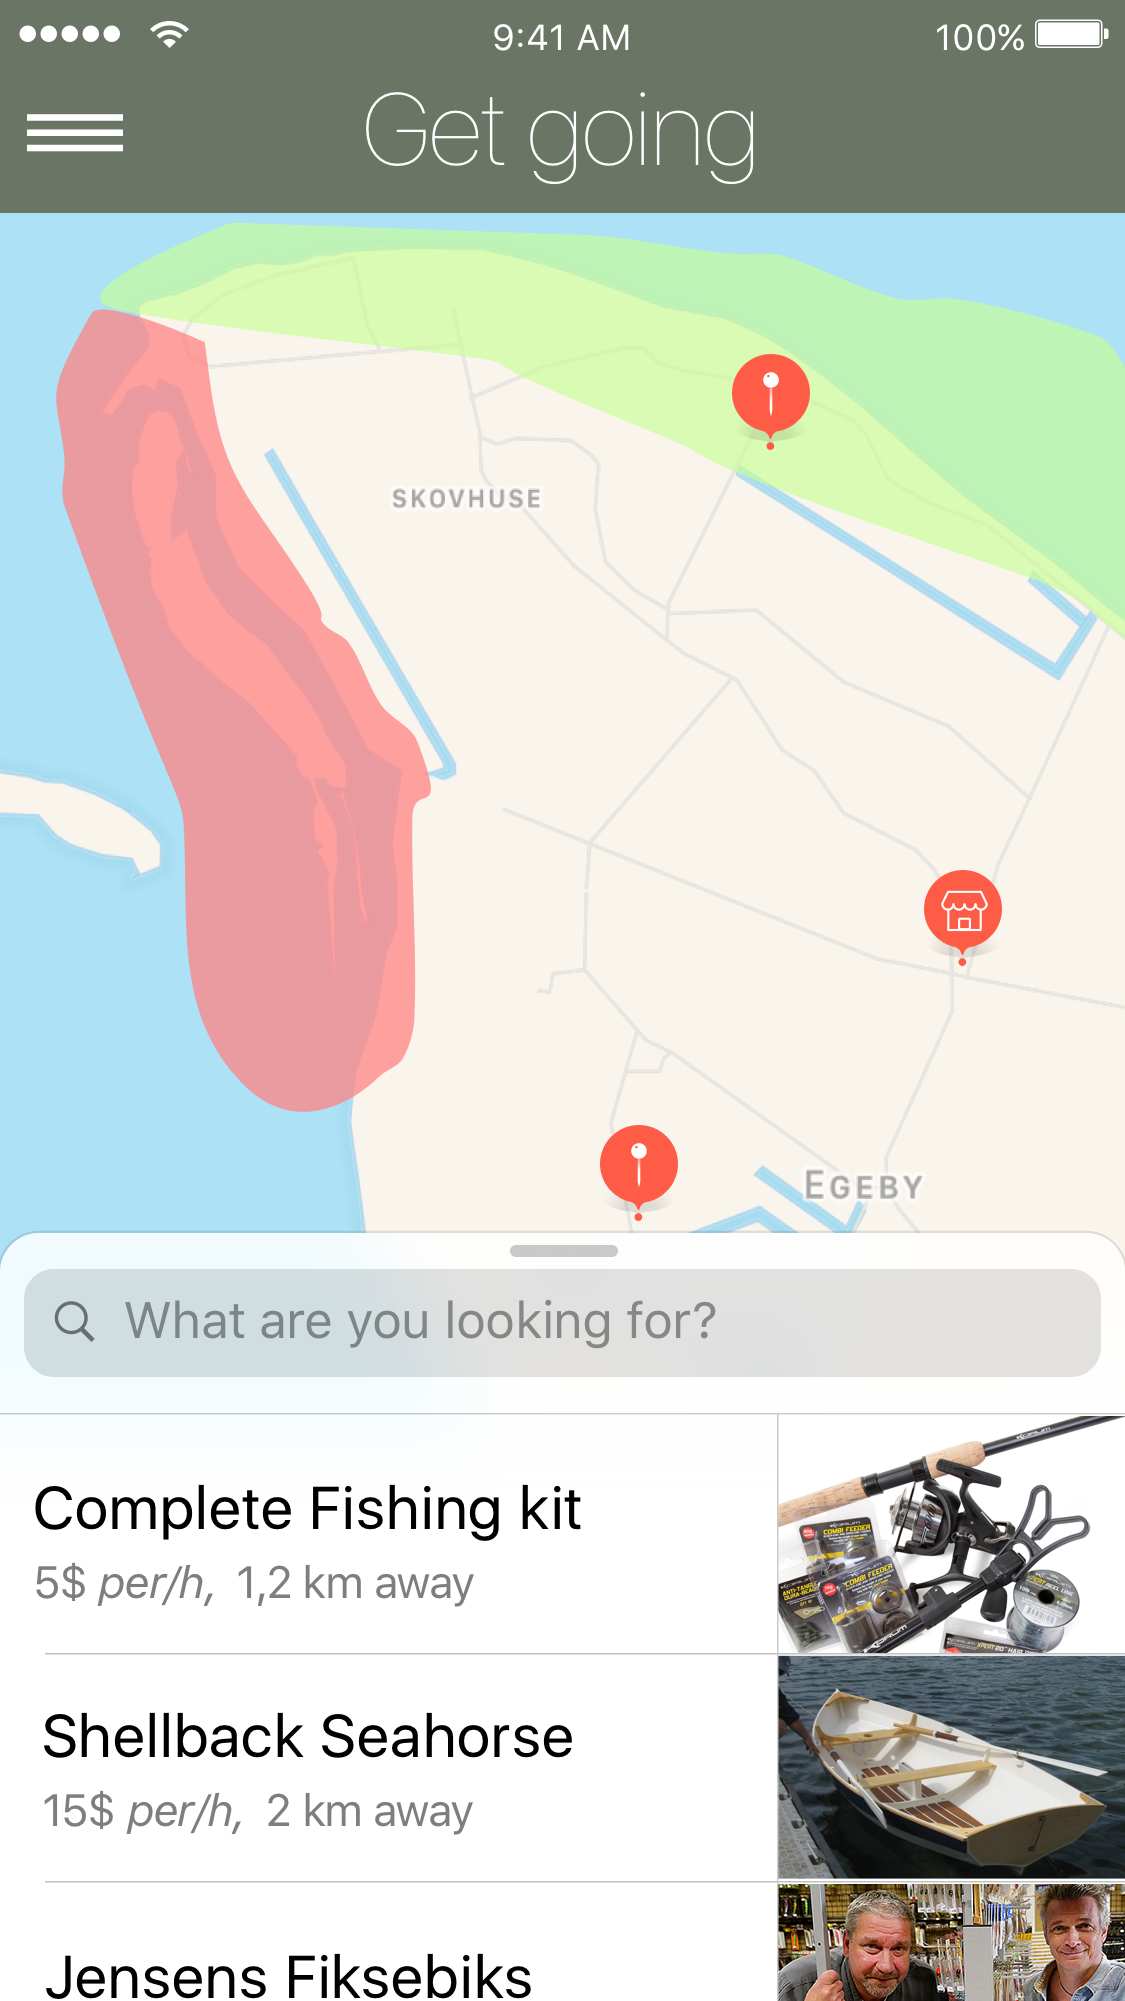
\includegraphics[width=0.4\textwidth]{images/Map.png}
  	  \label{fig:f2}
   	  \caption{Get going screen}
  \end{subfigure}
  \hfill
  \begin{subfigure}[t]{0.2\textwidth}
  	  \centering
  	  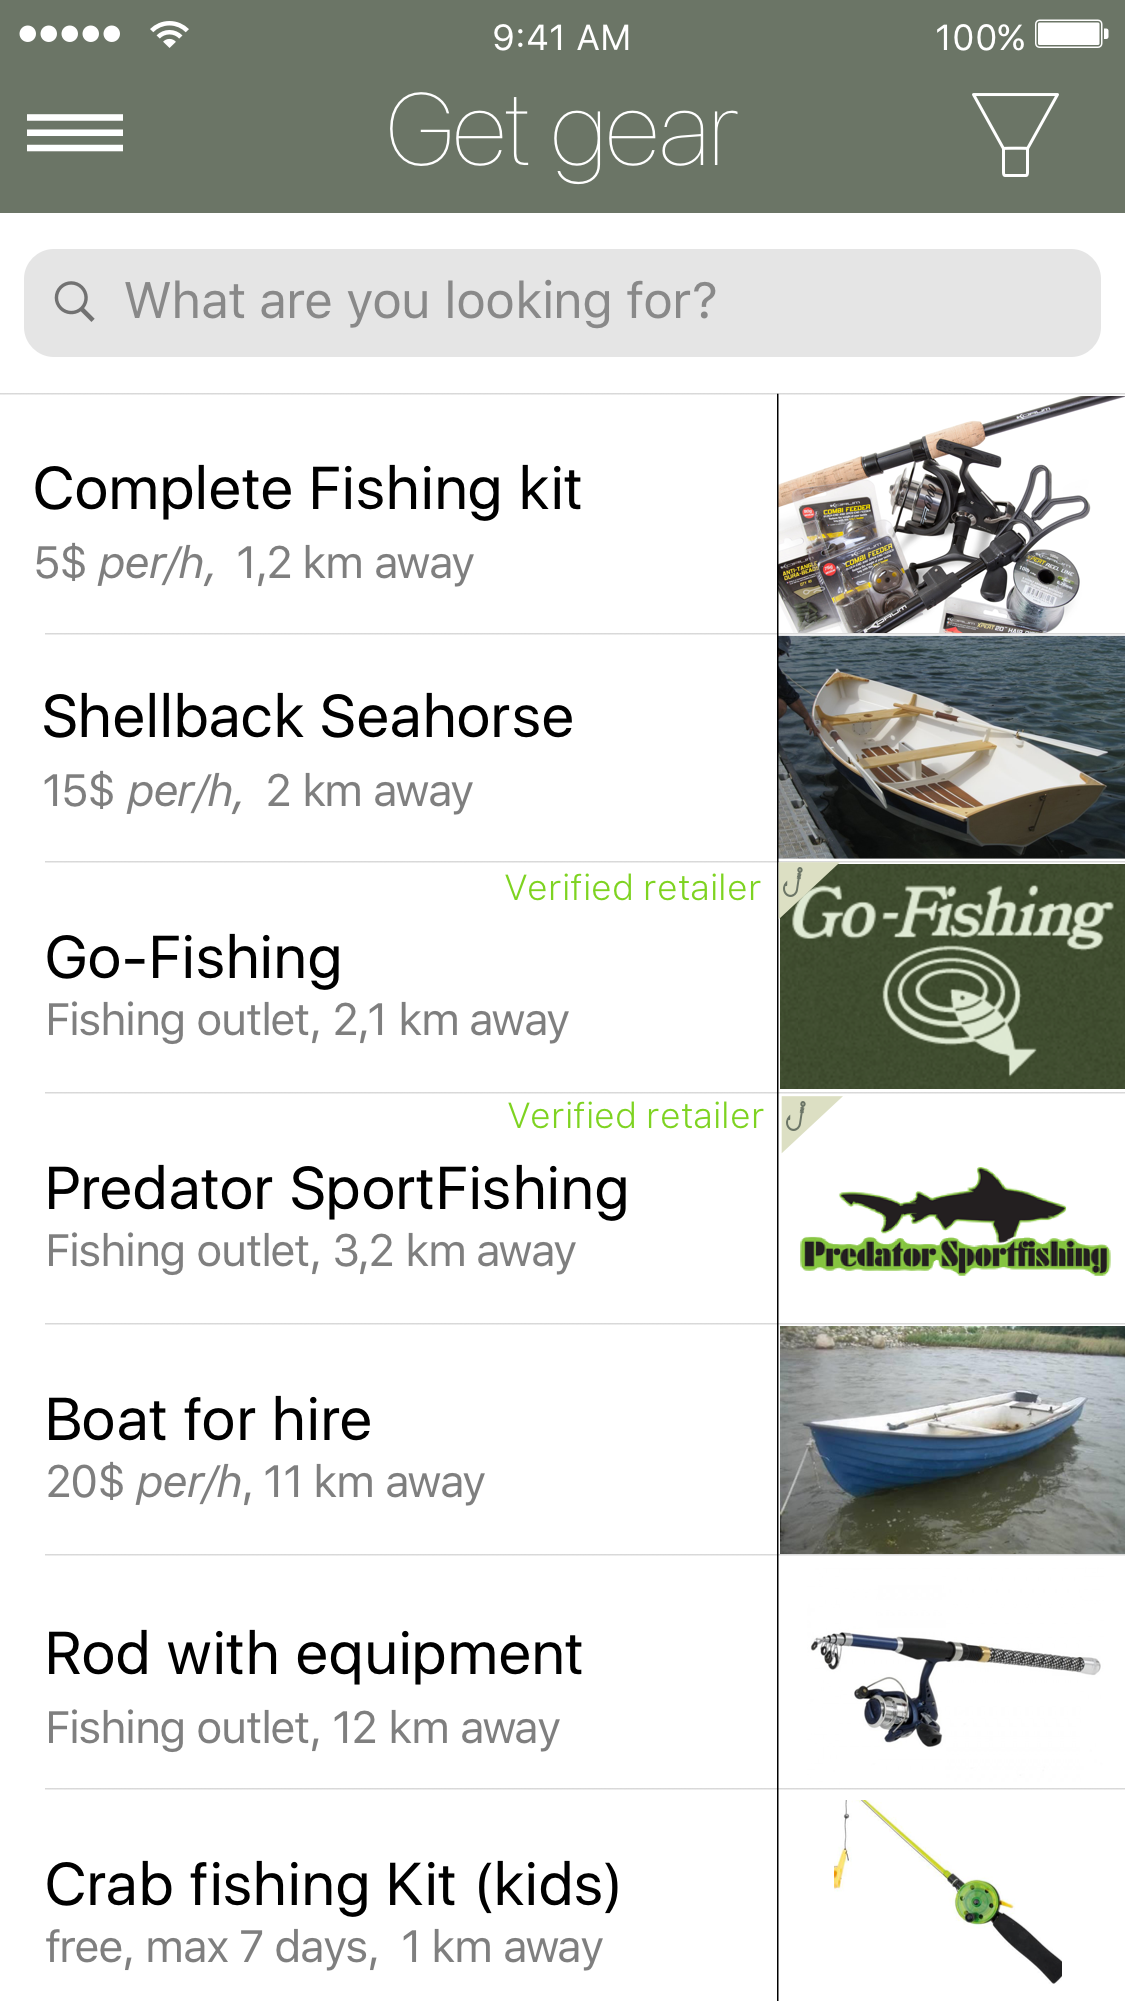
\includegraphics[width=0.4\textwidth]{images/Get_gear.png}
  	  \label{fig:f3}
   	  \caption{Get gear screen}
  \end{subfigure}  
  \hfill
  \begin{subfigure}[t]{0.2\textwidth}
  	  \centering
  	  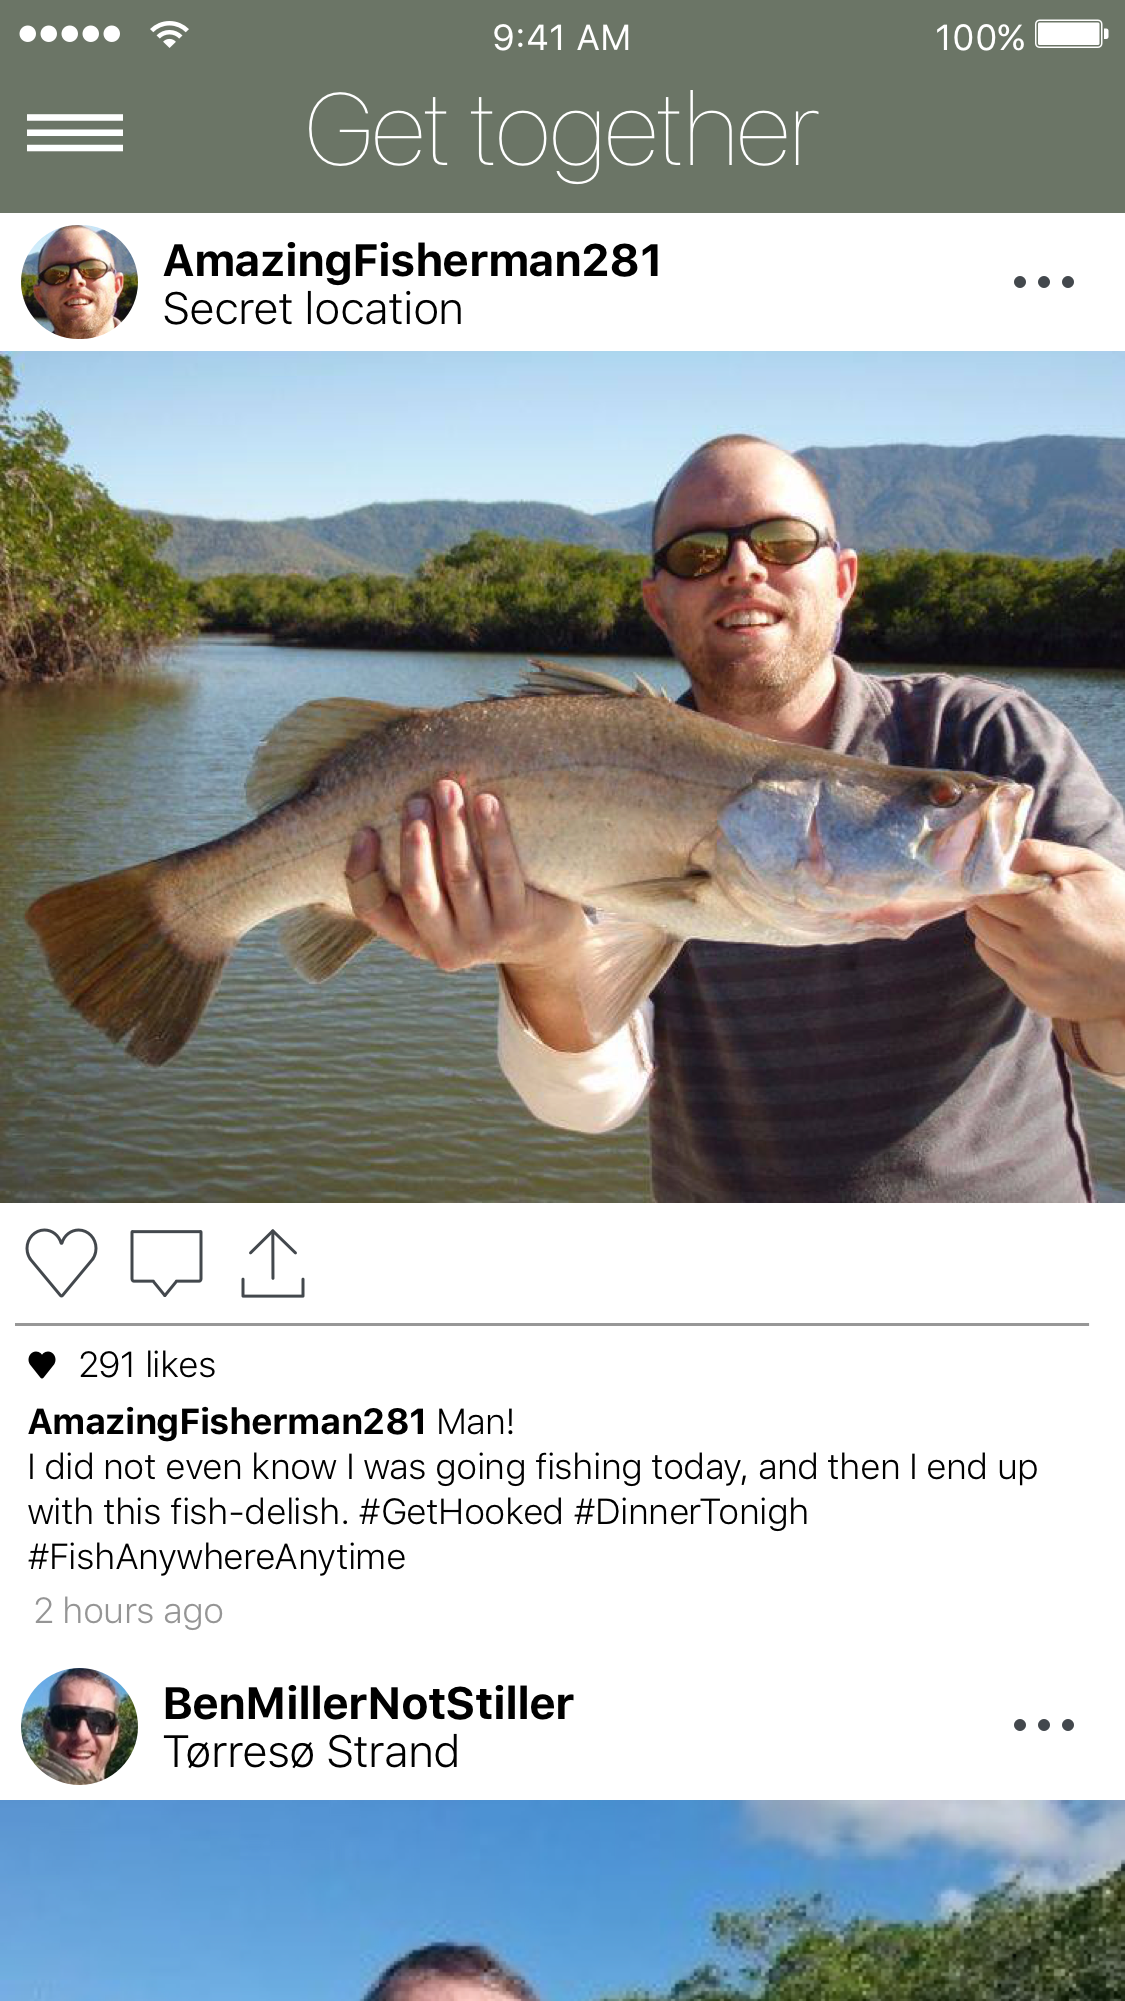
\includegraphics[width=0.4\textwidth]{images/Together.png}
  	  \label{fig:f4}
   	  \caption{Get Together}
  \end{subfigure}
  \hfill
  \newline
  \caption{Mockups of the application}
  \textit{See appendix \ref{app:mockups}, for larger versions}
 \end{figure*}

\begin{enumerate}[R1]
	\item The user should be able to login via. single sign on (such as Facebook and Google \cite{oauth}).
	\item The application should contain a map, showing the current location of the user.
	\item The application should display legal and nonlegal fishing areas on the map described in R02.
	\item The application should show, what the required fishing licence(s) is/are for the given area.
	\item The application should display owners of fishing equipment, who rents-out their	equipment on the map described in R02.
	\item The application should display fishing outlets, who rents out or sell equipment, on	the map described in R02.
	\item The application should contain a section, which gives the user information about fishing possibilities, in the area near them.
	\item The user should be able to rent equipment, from shops and owners.
	\item The application should contain a section introducing newcomers to the basics of fishing, either using a text or video format.
	\item The user should be able to acquire several valid fishing licences.
	\item The user should be able to renew expired or soon to be expired licenses \begin{enumerate}[R11.1]
	\item Optional: Automatic renewal \end{enumerate}
	\item The user should be able to see what kind of fish is the most likely to catch, in a certain area.
	\item The user should be able to see seasonal regulations, for catching certain species and size regulations.
	\item The user should be able to measure the length of a caught fish, using the camera of phone and a known-sized object as a reference of length.
	\item The user should be able to create events (e.g. a Fishing Tournament) for other users to attend.
	\item The user should be able to share what they caught, or their fishing experiences.
	\item The application should be developed for web and mobile platforms (IOS and Android)
\end{enumerate}